
%% ==================================================================================================
%%
\documentclass[12pt]{book}
\usepackage{amsfonts}
\usepackage{amsmath}
\usepackage{amssymb}
\usepackage{graphicx}
\usepackage{hyperref}
\usepackage{float}
\usepackage{verbatim}
\usepackage{xlop} %% for multiplication https://tex.stackexchange.com/questions/11702/how-to-present-a-vertical-multiplication-addition
\usepackage{listings} %% to format generic computer code
\usepackage{lmodern} % for bold teletype font
\usepackage{minted} % colour Java code

\usepackage{tasks}
%\NewTasks[style=enumerate,counter-format=tsk[A].,label-width=3ex]{choice}[\item](4)

%% =======   set page margins    =======
\setlength{\textheight}{10in}
\setlength{\textwidth}{7.4in}
\setlength{\topmargin}{-0.75in}
\setlength{\oddsidemargin}{-0.5in}
\setlength{\evensidemargin}{-0.5in}
\setlength{\parskip}{0.15in}
\setlength{\parindent}{0in}

%%  for European long division
% https://tex.stackexchange.com/questions/432435/how-to-set-up-european-french-style-long-division-in-tex
\newcommand\frdiv[5]{%
    \[
    \renewcommand\arraystretch{1.5}
    \begin{array}{l| l}
    #1 & #2 \\
    \cline{2-2}
    #3 & #4 \\
    \cline{1-1}
    #5 & \\
    \end{array}
    \]
}

%%  for European long division


%% ==================================================================================================

\begin{document}

%\title{ITI1100 Digital Systems I}
%\author{Kien Do 300163370}
%\date{Assignment \#1}
\newcommand{\reporttitle}{Laboratoire 4}
\newcommand{\reportauthorOne}{Kien Do}
\newcommand{\cidOne}{300163370}
\input{titlePage/titlepage.txt}



%% ==================================================================================================

%%%%%%%%%%%% PROBLEMS START HERE
\begin{enumerate}
    
    \item
    
    
\includegraphics[scale=0.5]{q1question.PNG}\\
    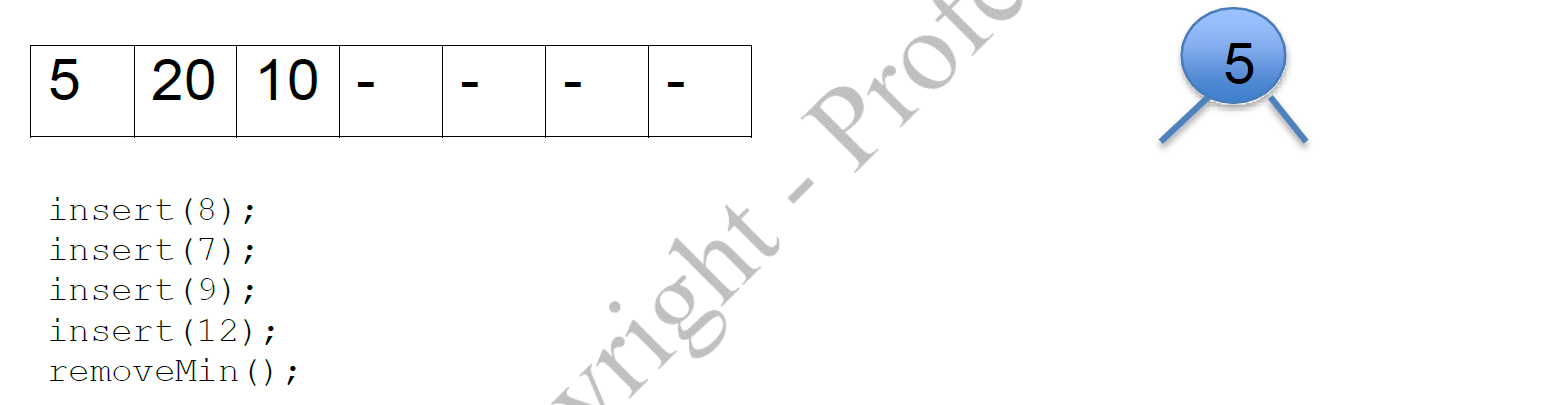
\includegraphics[scale=0.5]{q1question2.PNG}\\
    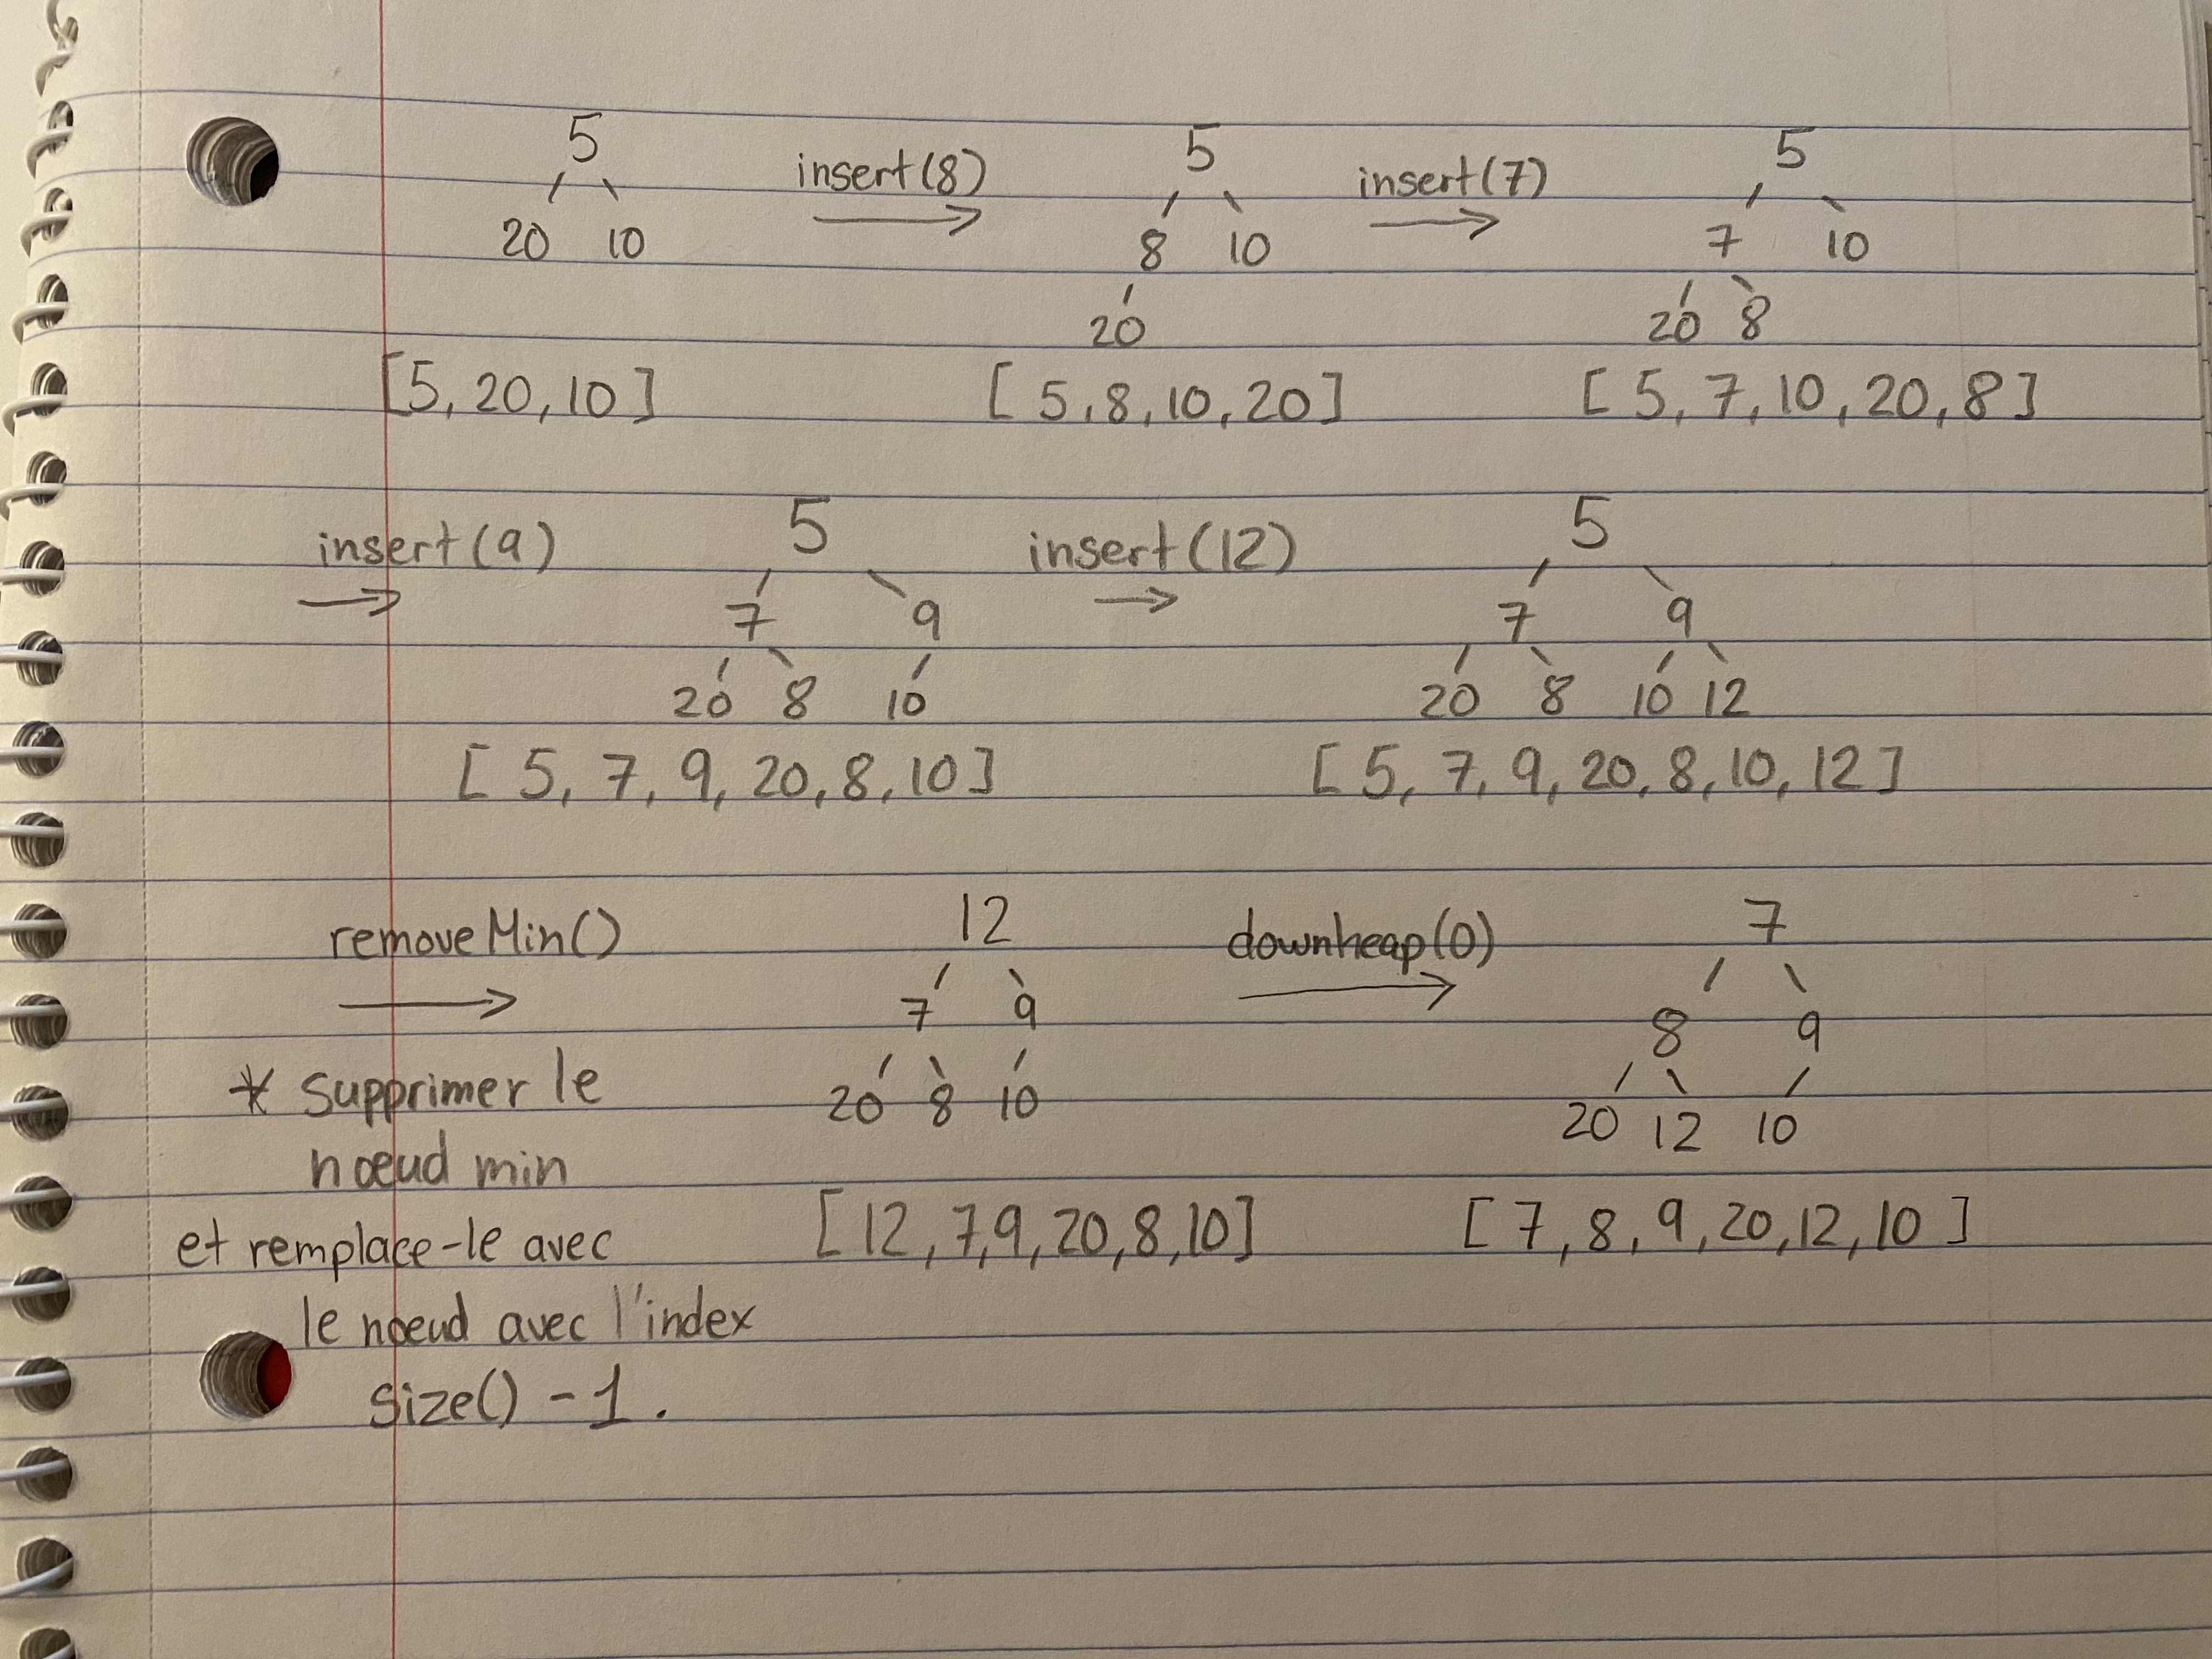
\includegraphics[scale=0.13]{q1answer.png}\\
    
    \newpage
    
    \item 
    
    
\includegraphics[scale=0.5]{q2question.png}\\
    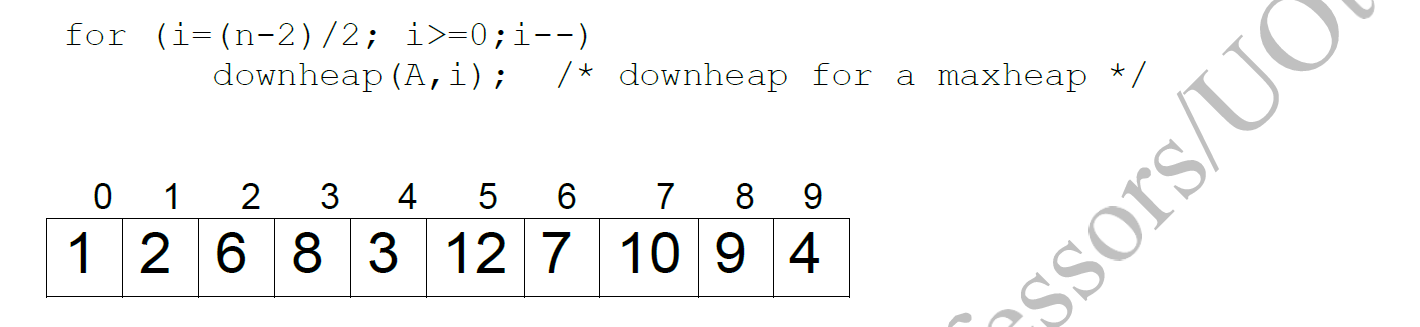
\includegraphics[scale=0.5]{q2question2.png}\\
    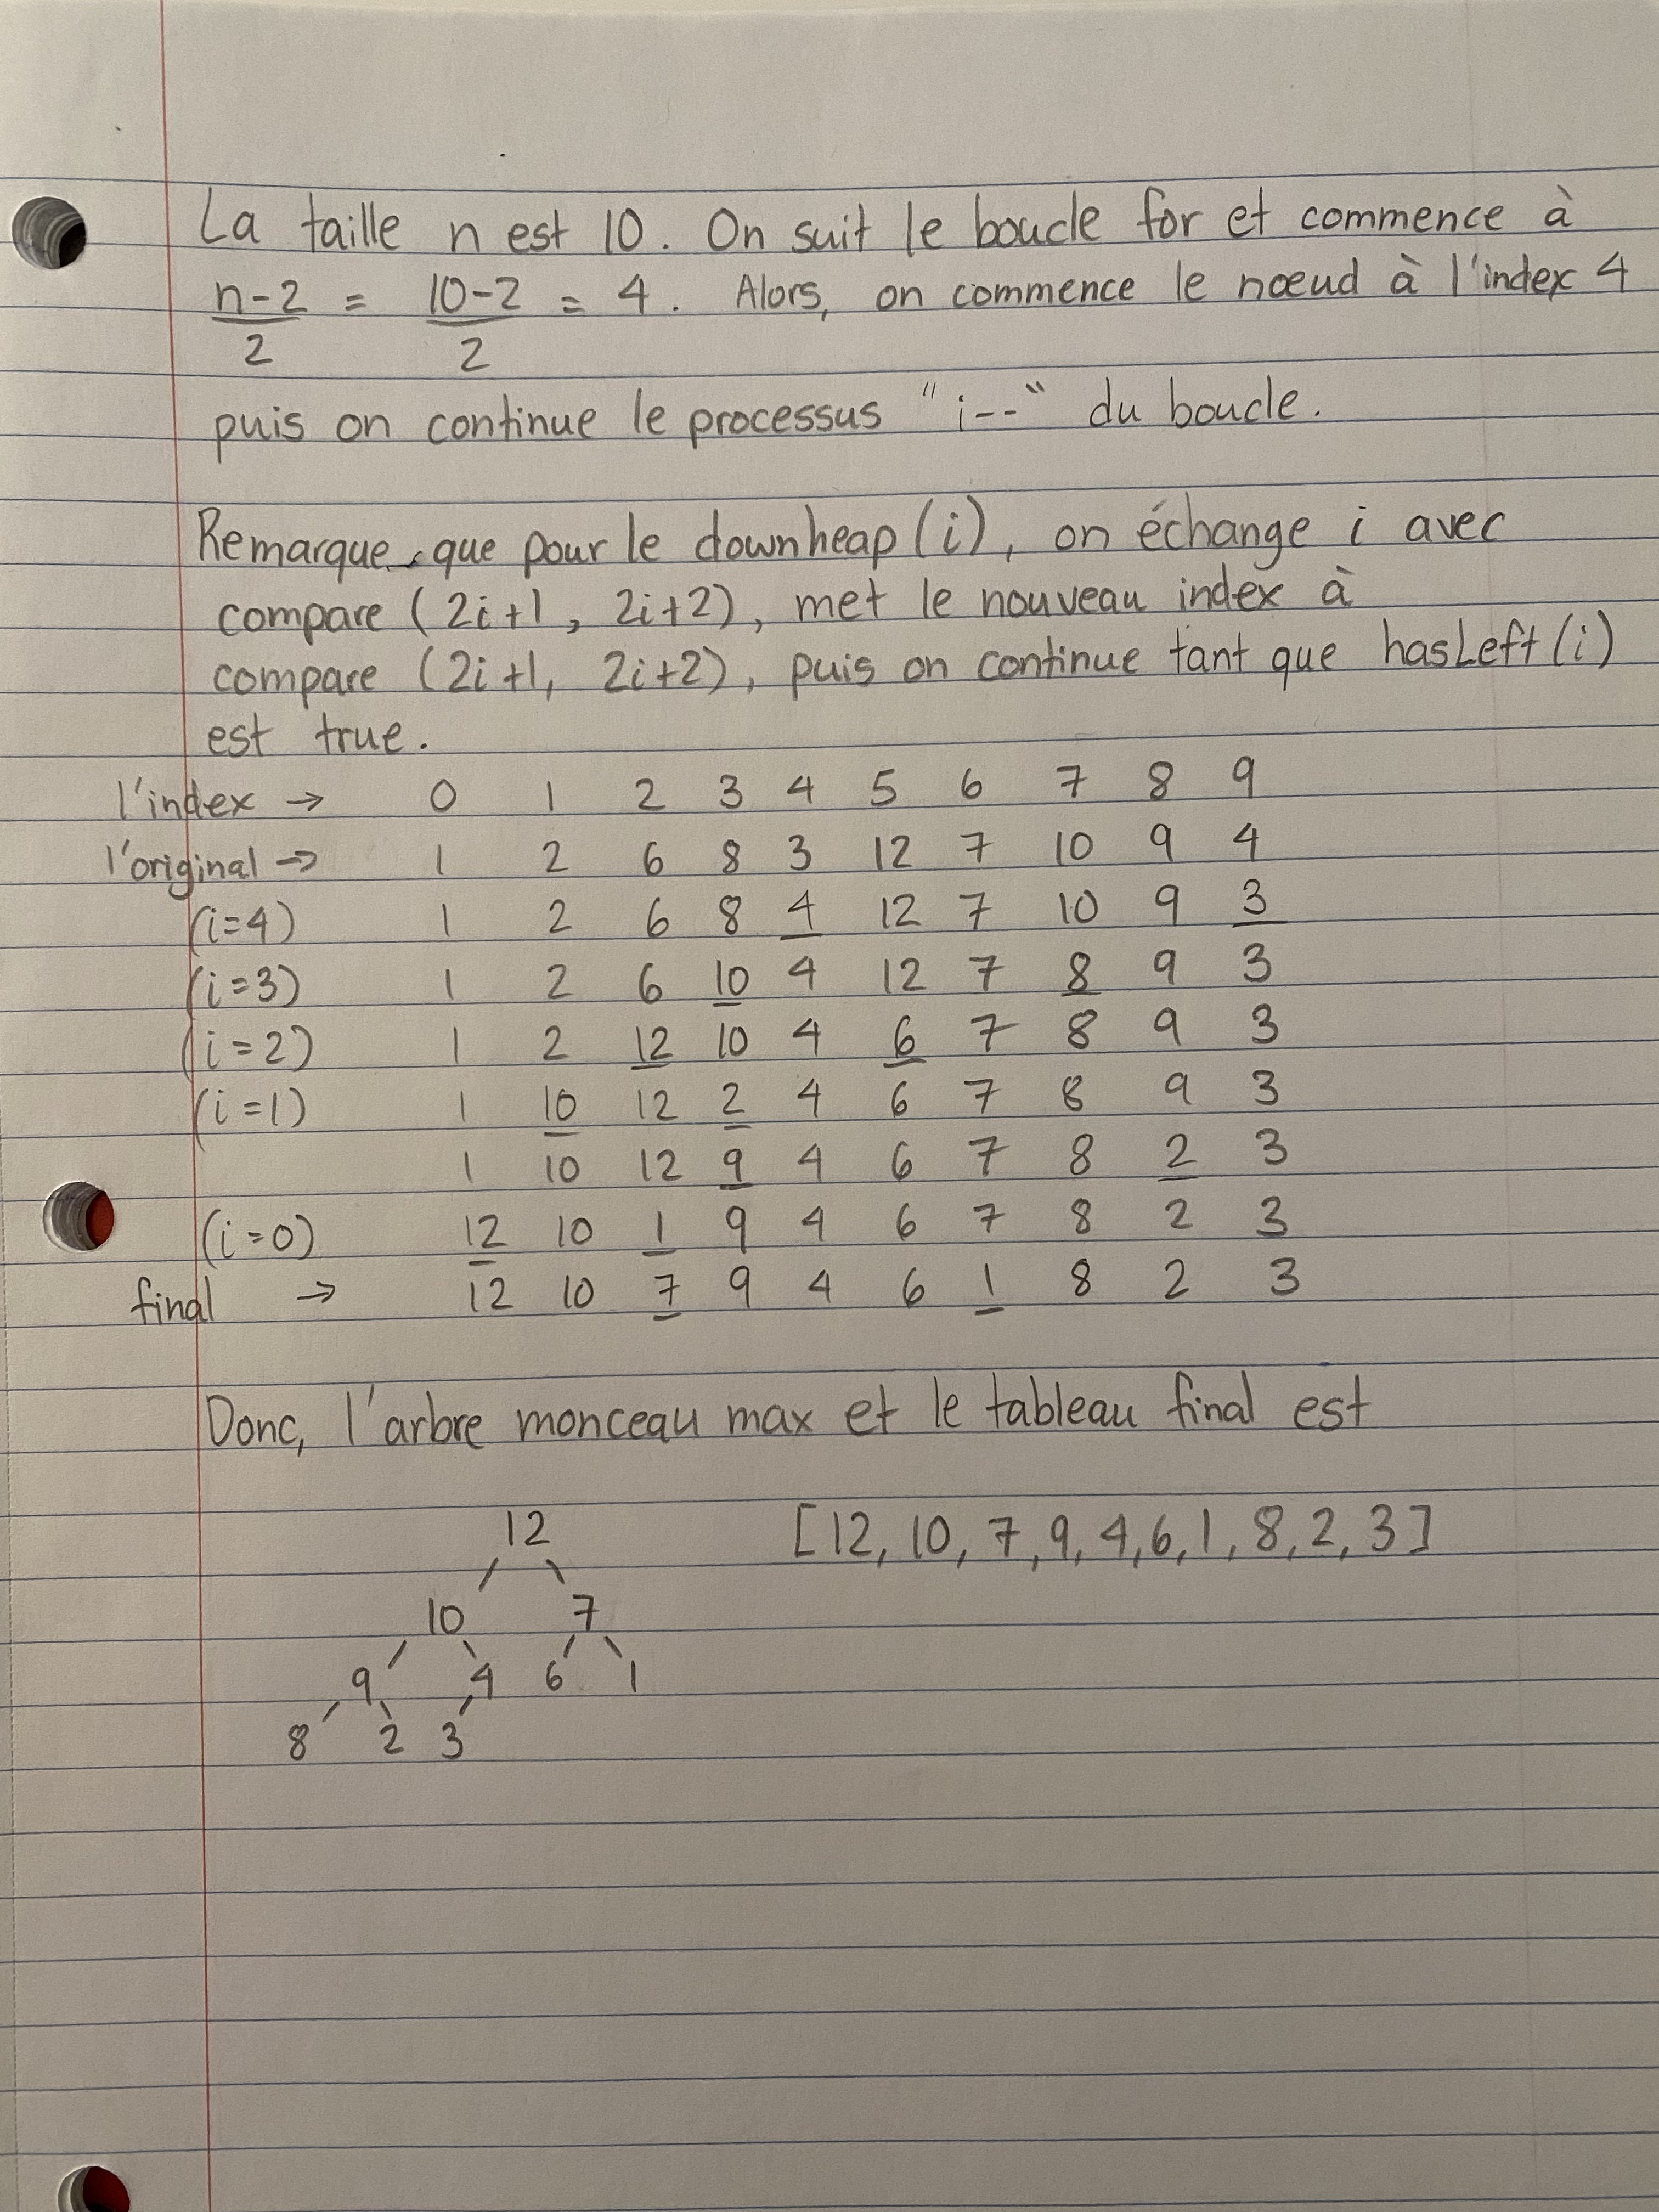
\includegraphics[scale=0.13]{q2answer.png}
    
    \newpage
    
    \item 
    
    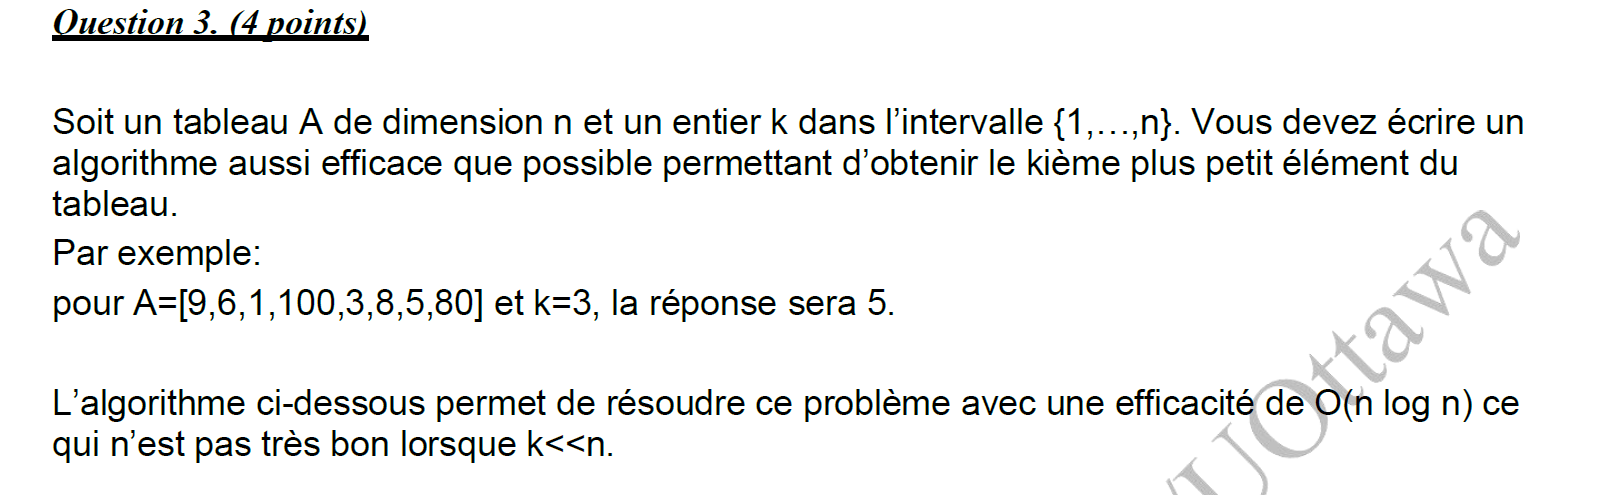
\includegraphics[scale=0.5]{q3question.png}\\
    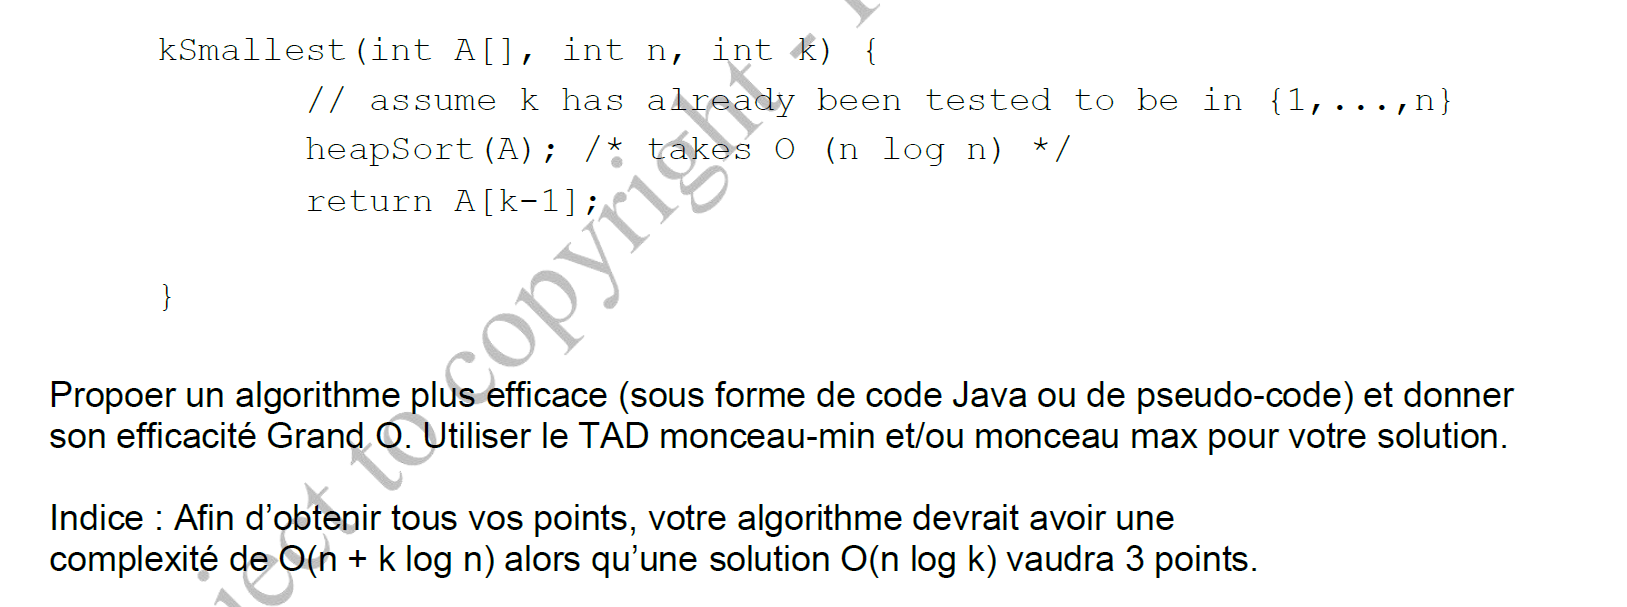
\includegraphics[scale=0.5]{q3question2.png}\\
    
    \begin{minted}[breaklines,frame=single]{java}
int kSmallest (int A[], int n, int k) {
    // assume k is between 1 and n, inclusive
    
    // build a min heap from the given array A
    Heap minHeap = new Heap(); // create empty min heap
    minHeap.buildMinHeap(A); // build min heap -> O(n)
    
    // get the kth smallest element
    int kthSmallestNum = 0;
    // call removeMin() k times -> O(k)
    for (int i = 0; i < k; i++) {
        kthSmallestNum = minHeap.removeMin(); // recall removeMin() is O(logn)
    }
    
    // This algorithm is O(n + k log(n))
    
    return kthSmallestNum;
}
        \end{minted}
    
    
\end{enumerate}





\end{document} 
